\subsection{Szenarios}
\label{sec:study-szenarios}
Die drei Szenarios der Usability-Studie sind so konzipiert, dass der Anspruch im Verlauf der Testsitzungen zunimmt. So sollte sichergestellt werden, dass die Teilnehmer:innen nicht mit zu vielen neuen Funktionalitäten auf einmal konfrontiert werden. Eckdaten zu den Szenarios können in Anhang \ref{app:handout} nachvollzogen werden, während Anhang \ref{app:scenarios} Bildschirmfotos des Block-Editors aus den Szenarios zeigt.

Das erste Szenario entspricht der Definition einer Konvertierung in Simplex4TwIS. Dabei soll eine Importtabelle, gefüllt mit Daten von Bundesländern, in das Realitätsmodell übertragen werden. Dazu wurden die Rohdaten bereits im Vorhinein in die Importtabelle geladen, und eine Objektklasse mit den benötigten Attributen erstellt. Da die Daten hier bereits alle im richtigen Format vorliegen, besteht die Konvertierung nur aus Zuweisungen der Spalten der Importtabelle zu den Attributen der Objektklasse.

Beim zweiten Szenario handelt es sich ebenso um eine Konvertierung, wobei die Quelldaten noch nicht vollständig im richtigen Format vorliegen. Die Teilnehmer:innen mussten einen zusammengesetzten Schlüssel erstellen und eine Punktgeometrie aus Längen- und Breitengrad unter der Verwendung von \texttt{ST\_MakePoint} anlegen. Des Weiteren mussten die Daten mit einem Filter ausschließlich auf Bundesländer reduziert werden. Das Filter-Feld stellt in diesem Szenario ein neues Konzept dar.

Im dritten Szenario soll der Block-Editor in der Bearbeitung von SimplexSzenarios getestet werden. Dazu wurde ein Beispiel mit drei Objektklassen gewählt: Adressen, Straßen und Ortsteile. Diese sollten von den Teilnehmer:innen zu einer Übersicht aller Adressen im Ortsteil Lindenau zusammengestellt werden. Die Attribute können von der Auswahl auf der linken Seite übernommen werden, müssen aber zunächst als neue Felder hinzugefügt und benannt werden. Sowohl das Benennen von Feldern, als auch das Zusammenstellen von Daten aus mehreren Objektklassen bilden hier neue Konzepte. Auch in diesem Szenario muss gefiltert werden.

Am Ende jedes Szenarios sollten die Teilnehmer:innen ihre Arbeit mit dem "Speichern"-Button oben rechts bestätigen. Dieser leitet zu einer Tabelle weiter, wie sie in Abbildung \ref{fig:scenario-result} zu sehen ist. In dieser Vorschauansicht können die konvertierten oder in SimplexSzenarios enthaltenen Objekte überprüft werden. Sollten Änderungen vonnöten sein, kann mit dem "Zurück"-Button zum Block-Editor zurück navigiert werden, und die zuvor getroffene Auswahl angepasst werden.

\begin{figure}
  \centering
  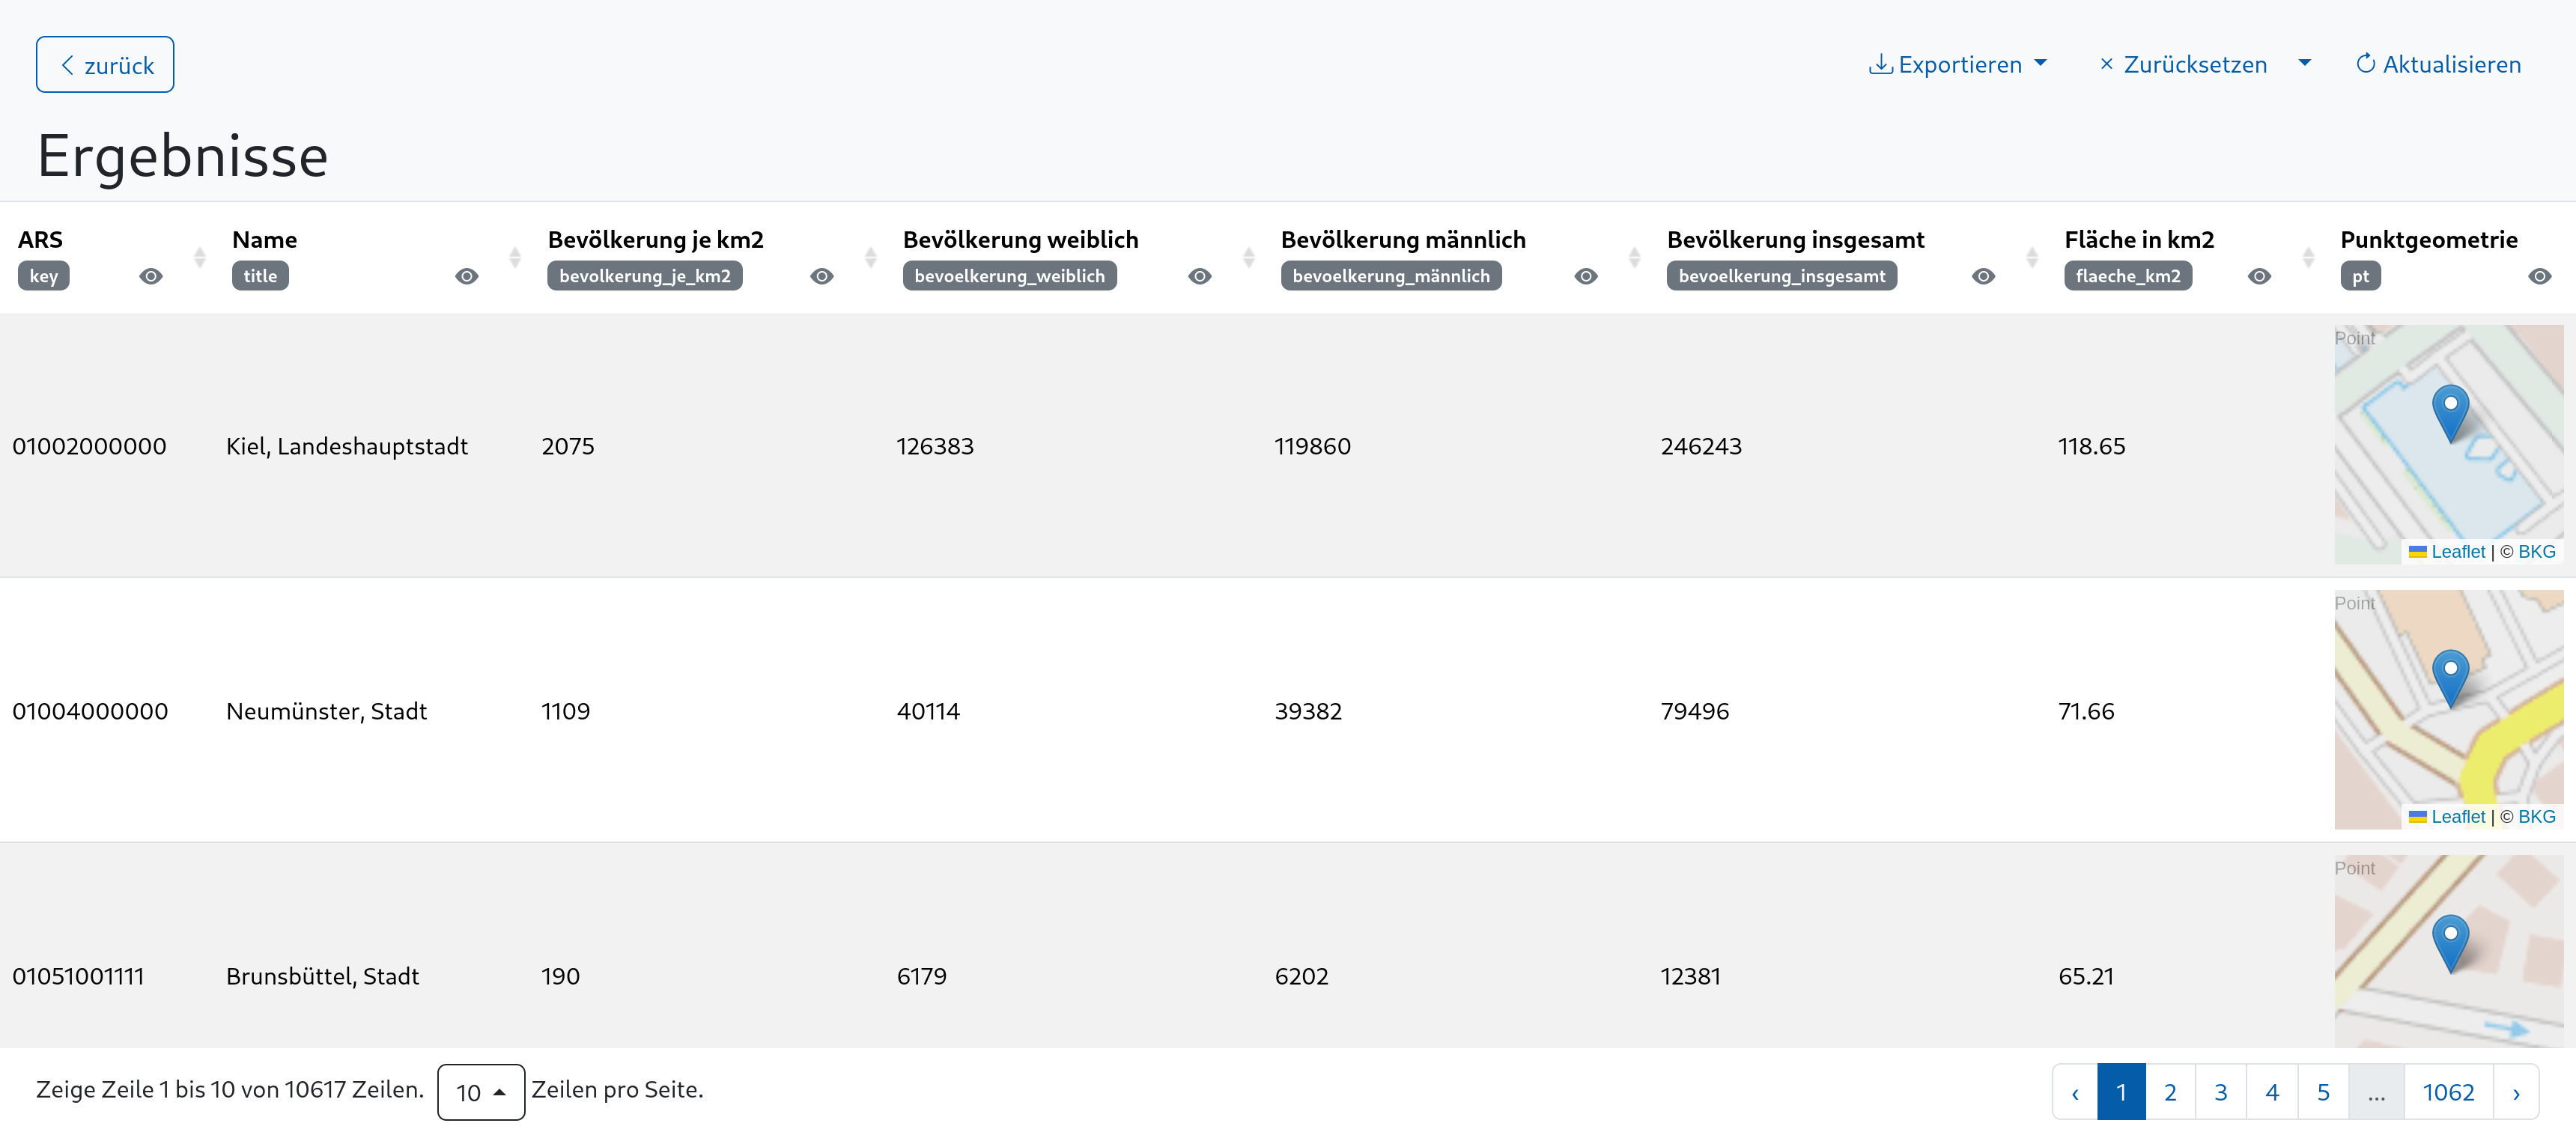
\includegraphics[width=.95\textwidth]{assets/results-szenario-2.png}
  \caption[Ergebnisstabelle am Ende des zweiten Szenarios.]{Abschluss des zweiten Szenarios: Es wird eine Tabelle mit den resultierenden Objekten angezeigt. Somit kann überprüft werden, ob alle benötigten Felder ausgefüllt sind, der zusammengesetzte Schlüssel \ac{ARS} angemessen definiert wurde und die Geometrie korrekt gebildet wurde.}
  \label{fig:scenario-result}
\end{figure}

